\documentclass[10pt, letterpaper]{article}
\usepackage[margin=0.75in]{geometry}
\usepackage{hyperref}
\usepackage{mathtools}
\usepackage{indentfirst}
\usepackage{graphicx}

\pagenumbering{gobble}
\setlength{\parindent}{-0.5cm}
\hypersetup{
    colorlinks   = true,
    urlcolor     = blue,
}

\newcommand*\rfrac[2]{{}^{#1}\!/_{#2}}

\title{Fiddler on the Proof - Sorting Hat}
\author{Alex Zhu}
\date{November 12, 2024}

\begin{document}
\maketitle

This is a solution to a Fiddler on the Proof \href{https://thefiddler.substack.com/p/where-will-the-sorting-hat-put-you}{puzzle}. \\

To make things easier to follow, let us suppose that Logwarts' four houses are:
\begin{itemize}
    \item Graphindor (hence referred to as $\mathcal{G}$)
    \item Riemannclaw (hence referred to as $\mathcal{R}$)
    \item Hexapuff (hence referred to as $\mathcal{H}$)
    \item Scalerin (hence referred to as $\mathcal{S}$)
\end{itemize}

Suppose that for some arbitrary round $S$, the probability of a student being sorted into $\mathcal{G}$ is $P_s$.\\

Now let us work through round $S+1$.

If the student $S$ was placed into $\mathcal{G}$, then, by the rules, student $S+1$ cannot be a $\mathcal{G}$. So we can disregard this case.

On the other hand, suppose student $S$ was placed into one of the other housees - let's denote that as $\mathcal{X}$, which may be any of $\mathcal{R}$, $\mathcal{H}$, $\mathcal{S}$.
\begin{itemize}

\item
    This student has a $\rfrac{1}{4}$ chance of choosing $\mathcal{G}$, which is allowed.
\item
    However, this student also has a $\rfrac{1}{4}$ chance of choosing $\mathcal{X}$ again, which is not allowed.
    So that's s a $\rfrac{1}{3}$ chance of the hat placing them in $\mathcal{G}$ against their will, for a total of $\rfrac{1}{4}*\rfrac{1}{3}=\rfrac{1}{12}$ chance of $\mathcal{G}$ given that the previous student $S$ was not placed into $\mathcal{G}$.
\item
    The remaining $\rfrac{1}{2}$ chance is that the student picks one of the other two non-$\mathcal{G}$ and non-$\mathcal{X}$. This is allowed and doesn't contribute to the odds of student $S+1$ ending up in $\mathcal{G}$.
\end{itemize}

So, if student $S$ is placed into $\mathcal{X}$, the chances of student $S+1$ being placed into $\mathcal{G}$ are
$\rfrac{1}{4} + \rfrac{1}{12} = \rfrac{1}{3}$.\\

We know the odds of student $S$ being placed into $\mathcal{X}$ to be $1-P_s$, and we can disregard the $P_s$ case as impossible for student $S+1$ to be a $\mathcal{G}$, so that means that:
\begin{equation*}
    P_{s+1} = \rfrac{1}{3}(1 - P_s)
\end{equation*}

Let's fruther define $B_s$ as the chances that our protagonist Barry Plotter gets his choice, given that he is $S_{th}$ in line.
Since Barry chooses $\mathcal{G}$, he will get his wish as long as student $S-1$ doesn't pick $\mathcal{G}$. So:
\begin{equation*}
    B_s = 1 - P_{s-1}
\end{equation*}

We can plug this into Excel (okay, Google Sheets) to get our results:\\

\begin{tabular}{l | l | l }
    Round   & $P_s$     & $B_s$ \\ \hline
    1       & 1.0000    & n/a (Barry can't be first)\\
    2       & 0.0000    & 0.0000 \\
    3       & 0.3333    & 1.0000 \\
    4       & 0.2222    & 0.6667 \\
    5       & 0.2593    & 0.7778 \\
    6       & 0.2469    & 0.7407 \\
    7       & 0.2510    & 0.7531 \\
    8       & 0.2497    & 0.7490 \\
    9       & 0.2501    & 0.7503 \\
    10      & 0.2500    & 0.7499 \\
\end{tabular}\\

So our solution is $B_{10} = 74.9886\%$.

\section*{Extra Credit}

Define $W_m$ as the odds that Barry gets into $\mathcal{G}$ given that he wakes up at student $M$ getting sorted
and $E_n$ as Barry's overall chances to get into $\mathcal{G}$ given he is $N^{th}$ in line.\\

If Barry wakes up when student $M$ is being sorted, the problem is identical to the original prompt, except now we're starting from student $M$ instead of student $1$.
So it follows that:
\begin{equation*}
    W_m = B_{n-m}
\end{equation*}

By the prompt, $M$ is $[1..N-1]$. So $W_m$ ranges from $B_{n-1}$ to $B_{n-(n-1)} = B_1$.\\

Every value in $M$ has an equal chance to be chosen, so $E_n$ is simply the average of every value $(B_1..B_{n-1})$. Plug this back into Google Sheets and the table starts:\\

\begin{tabular}{l | l | l | l }
    Round   & $P_s$     & $B_s$     & $E_n$     \\ \hline
    1       & 1.0000    & n/a       & n/a       \\
    2       & 0.0000    & 0.0000    & 0.0000    \\
    3       & 0.3333    & 1.0000    & 0.5000    \\
    4       & 0.2222    & 0.6667    & 0.5556    \\
    5       & 0.2593    & 0.7778    & 0.6111    \\
    6       & 0.2469    & 0.7407    & 0.6370    \\
    7       & 0.2510    & 0.7531    & 0.6564    \\
    8       & 0.2497    & 0.7490    & 0.6696    \\
    9       & 0.2501    & 0.7503    & 0.6797    \\
    10      & 0.2500    & 0.7499    & 0.6875    \\
\end{tabular}\\

We continue a while until finally $E_n > p$ at $N = 4922$.

\pagebreak
\section*{Graphs}

We can see that Barry's overall odds quickly approach $\rfrac{3}{4}$, which makes sense for earlier rounds to matter less and less.

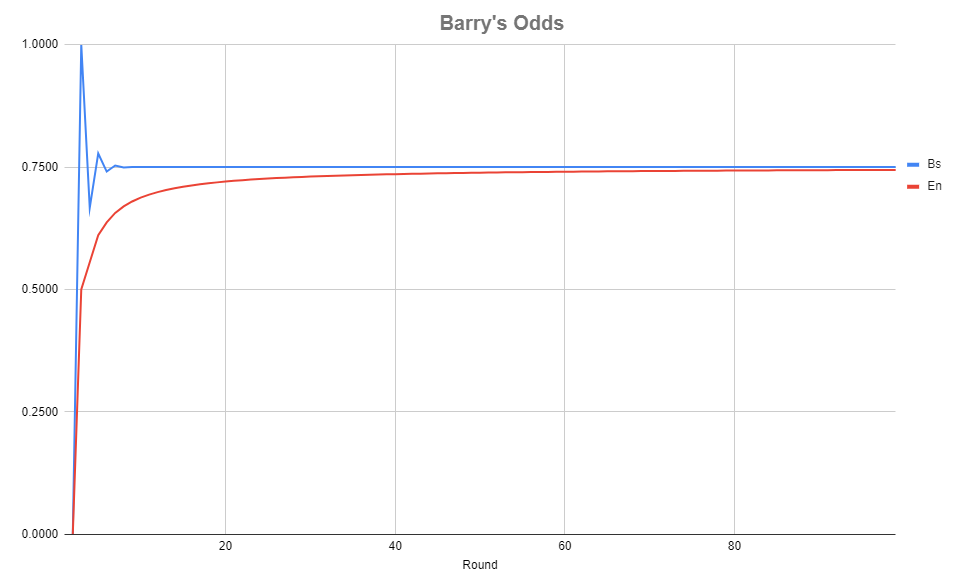
\includegraphics[height=10cm]{sorting_hat_01.png}

We can also see just how long it takes the extra credit scenario to reach just the 10th iteration if only Barry had gotten a better night's sleep.

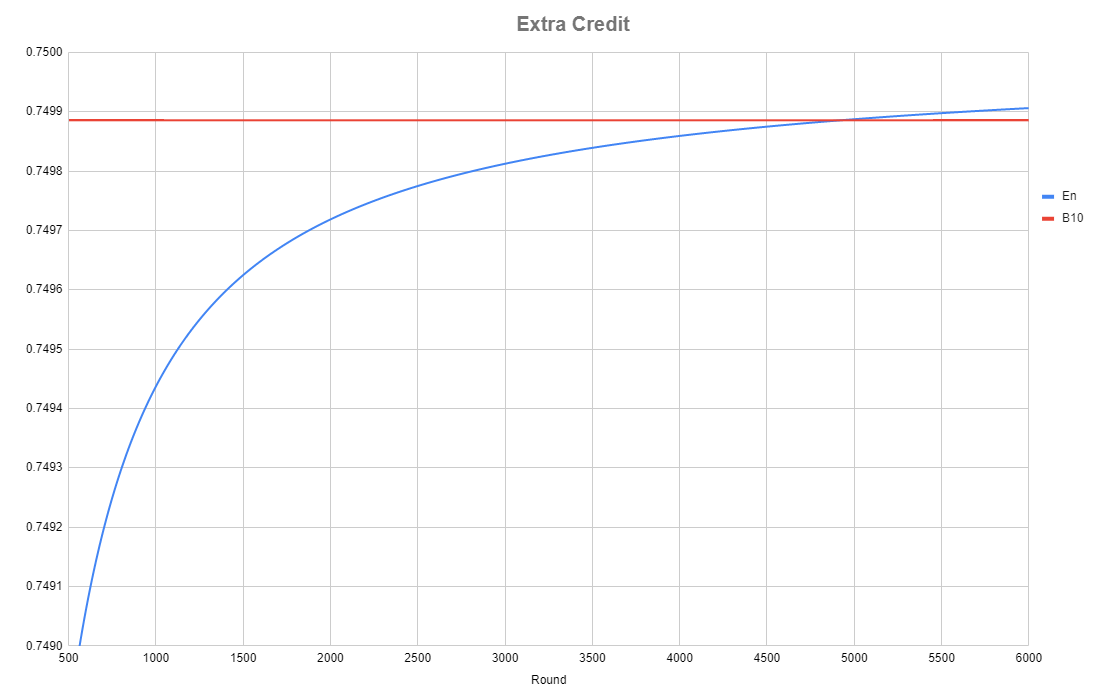
\includegraphics[height=10cm]{sorting_hat_02.png}

\end{document}